\documentclass[a1paper, landscape, fontscale=0.9]{baposter}
\usepackage[english]{babel}
\usepackage{csquotes}
\usepackage[scaled]{helvet}
\usepackage{titling}
\usepackage{url}
\usepackage{xcolor}
\usepackage{media9} 
\usepackage[rightcaption]{sidecap}
\usepackage{graphicx}
\usepackage{wrapfig}
\graphicspath{{diagrams/}{codeimages/}{listings/}}
\usepackage{amsmath}
\usepackage{amssymb}
\usepackage{multicol}
\usepackage[scaled]{helvet}
\usepackage{listings}

\title{Regular Polytopes : Code Dissection}
\author{Rob Nicolaides
        (School of Mathematics and Statistics, University of Sheffield)\\[0.5ex]
        Burkill summer studentship, under the supervision of Dr.\ James Cranch
        (contact: \texttt{J.D.Cranch@sheffield.ac.uk})}

% Sheffield logo blue
\definecolor{dblue}{rgb}{0.25,0.317,0.6}
\definecolor{lblue}{rgb}{0.11,0.753,0.929}

\newcommand{\bR}{\mathbb{R}}

\begin{document}
\begin{poster}{
    background=plain,
    bgColorOne=black!5,
    eyecatcher=false,
    borderColor=lblue,
    headerColorOne=dblue,
    textborder=rounded,
    headerborder=closed,
    headershape=rounded,
    headershade=plain,
    boxshade=plain,
    headerFontColor=white,
    boxColorOne=white,
    boxshade=plain}
{}
{\Huge\fontsize{50}{60}\selectfont\textsf{\thetitle}\vspace{0.2em}}
{\textsf{\theauthor}}
{
\includegraphics[bb=0 -40 502 250,height=0.12\textheight]{sheffield-logo}}

%%%%%%%%%%%%%%%%%%%%%%%%%%%%%%%%%%%%%%%%%%%%%%%%%%%%%%%%%%%%%%%%%%%%%%%%%%%%%%%%%%%%%%%%%%%%%%%

\headerbox{Summary}{name=summary,column=0}{
  This poster exhibits a library of \emph{Python 2} code created to
  manipulate polytopal tilings in one, two, three and four dimensions.

  %%% picture of 1D
  %%% picture of 2D
  %%% picture of 3D
  %%% picture of 4D
}

%%%%%%%%%%%%%%%%%%%%%%%%%%%%%%%%%%%%%%%%%%%%%%%%%%%%%%%%%%%%%%%%%%%%%%%%%%%%%%%%%%%%%%%%%%%%%%%

\headerbox{Linear algebra}{name=linear_algebra, column=0, below=summary}{

  \begin{minipage}{0.66\textwidth}
  There are \texttt{Vector2}, \texttt{Vector3} and \texttt{Vector4}
  classes, together with \texttt{Matrix2}, \texttt{Matrix3} and
  \texttt{Matrix4} classes. These are equipped with a full set of
  linear algebra methods.

  Of special interest are functions for generating random orthogonal
  matrices and random unit vectors (such as \texttt{random\_norm1},
  illustrated here).
  
  \begin{center}
    \includegraphics[scale=0.8]{norm1}
  \end{center}
  \end{minipage}
  \hfil
  \begin{minipage}{0.3\textwidth}
  \begin{center}
    \includegraphics[width=0.95\textwidth]{unit_ball}
  \end{center}
  \end{minipage}
}

%%%%%%%%%%%%%%%%%%%%%%%%%%%%%%%%%%%%%%%%%%%%%%%%%%%%%%%%%%%%%%%%%%%%%%%%%%%%%%%%%%%%%%%%%%%%%%%

\headerbox{Tilings}{name=core_code, column=0, below=linear_algebra}{

  The tiling classes are the core of the project. We have
  \texttt{Tiling1}, \texttt{Tiling2}, \texttt{Tiling3} and
  \texttt{Tiling4} classes for representing tilings of line segments
  in $\bR^1$, polygons in $\bR^2$, polyhedra in $\bR^3$ and polytopes
  in $\bR^4$ respectively.

  There are functions \texttt{tiling1}, \texttt{tiling2},
  \texttt{tiling3}, and \texttt{tiling4} for constructing them.
}

%%%%%%%%%%%%%%%%%%%%%%%%%%%%%%%%%%%%%%%%%%%%%%%%%%%%%%%%%%%%%%%%%%%%%%%%%%%%%%%%%%%%%%%%%%%%%%%

\headerbox{Convex hulls}{name=convex_hull,column=0, below = core_code}{

  It is common to specify a convex polytope as the convex hull of its
  vertices, and we give code to recover the higher structure from the
  vertices.

  We describe it in three dimensions for convenience, though we mostly
  use the generalisation to four dimensions.

  Firstly, we can tell whether three non-collinear vertices lie on a
  face of the convex hull: they do if and only if all simplices
  featuring those three vertices have the same sign to their signed
  volume (this sign tells you which side of the plane determined by
  those three vertices they are).

  A face is then a maximal set of coplanar vertices with the property
  that any three lie on a face.

  %%% Define dodecahedron, or similar

  This is used in our code to construct the regular four-dimensional
  polytopes; for the larger ones, it takes some considerable time to
  execute and so the results are stored.
}

%%%%%%%%%%%%%%%%%%%%%%%%%%%%%%%%%%%%%%%%%%%%%%%%%%%%%%%%%%%%%%%%%%%%%%%%%%%%%%%%%%%%%%%%%%%%%%%

\headerbox{Restriction Code}{name=restriction,column=0, below = convex_hull}{
Here we take a tiling object of $n$ dimensions and intersect in with hyper-plane $z = 0$ to create a tiling object of $(n-1)$ dimensions. This works by finding all the edges that have an intersection through the hyper-plane $z = 0$ and storing the point of intersection as a new vertex. Then it joins these verticies if the edges that they are of the intersection of are part of a common face. It joins these edges if the faces that they are of the intersection of are part of a common volume and so on.
\par \quad \par 
It complains if any vertices have $z = 0.$ 
Of course, this should be a measure-zero event, and can be avoided by small translations. 
This makes the algorithm much simpler: 
edges in the input produce vertices in the output, and faces in the input produce edges in the output. 
\par \quad \par 

Here is a sample of the code for taking a 2D cross-section of a 3D polyhedron. 

}

%%%%%%%%%%%%%%%%%%%%%%%%%%%%%%%%%%%%%%%%%%%%%%%%%%%%%%%%%%%%%%%%%%%%%%%%%%%%%%%%%%%%%%%%%%%%%%%

\headerbox{Periodic Tilings}{name=periodic, column=0, below=restriction}{

  \begin{minipage}{0.39\textwidth}
  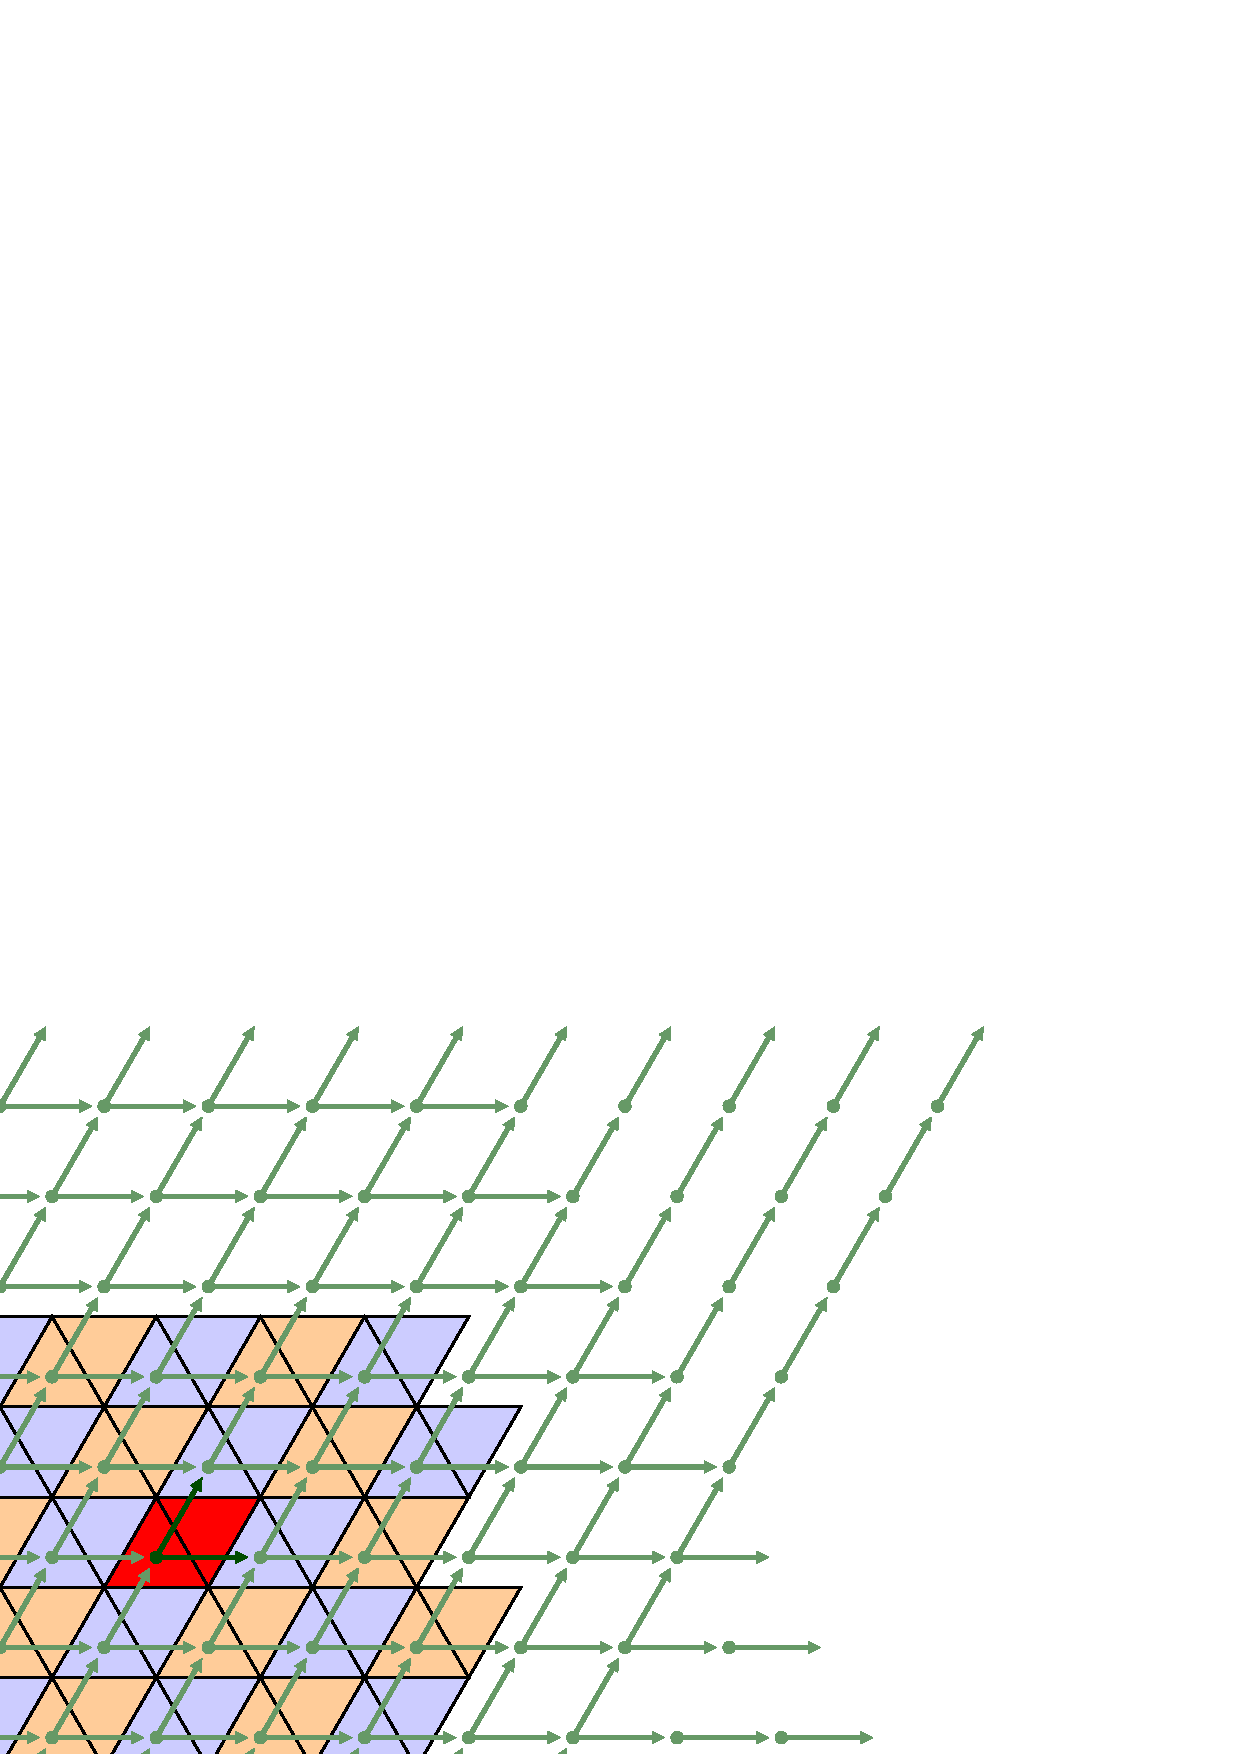
\includegraphics[width=0.95\textwidth]{fundamental}
  \end{minipage}
  \hfil
  \begin{minipage}{0.60\textwidth}
    There are two sets of functions for creating periodic tilings, and
    below we see some code which creates the periodic tiling depicted
    on the left.

    In both we need to specify the \emph{period vectors}: those
    vectors where translation gives a symmetry of the tiling. The
    tiling on the left has two period vectors shown in dark green.

    In both we also need to specify a \emph{fundamental domain}: the
    structure which must be copied along those period vectors in order
    to obtain the whole tiling. The tiling on the left has a
    fundamental domain in dark red, with its copies in light blue and
    salmon pink.

    In one approach (below), we specify precisely the fundamental
    structure: the tiling on the left has a single fundamental vertex,
    three fundamental edges (a horizontal and two diagonals), and two
    fundamental faces (the upwards-pointing and downwards-pointing
    triangles).

    The other is clumsier, and we give the fundamental domain as a
    tiling object, which means that some fundamental structure will be
    repeated: this must be detected and removed.
  \end{minipage}
  
  \begin{center}
    \includegraphics[scale=0.8]{triangles}
  \end{center}
}

\headerbox{Intersection Dissection}{name=restriction, column=0, below=periodic}{

}

\headerbox{Cartesian products}{name=cartesian, column=0, below=restriction}{

}


\end{poster}
\end{document}
